\documentclass[tikz,convert={outfile=\jobname.svg}]{standalone}
\usepackage{amsmath}
\usetikzlibrary{fit,backgrounds}
\usepackage{siunitx}	
\newcommand{\ddt}[1]{\ensuremath\frac{\mathrm{d}#1}{\mathrm{d}t}}
\newcommand{\eg}{\mbox{e.g.,\,}}
\newcommand{\ie}{\mbox{i.e.,\,}}
\usepackage{bm}
%\usetikzlibrary{...}% tikz package already loaded by 'tikz' option
\begin{document}
	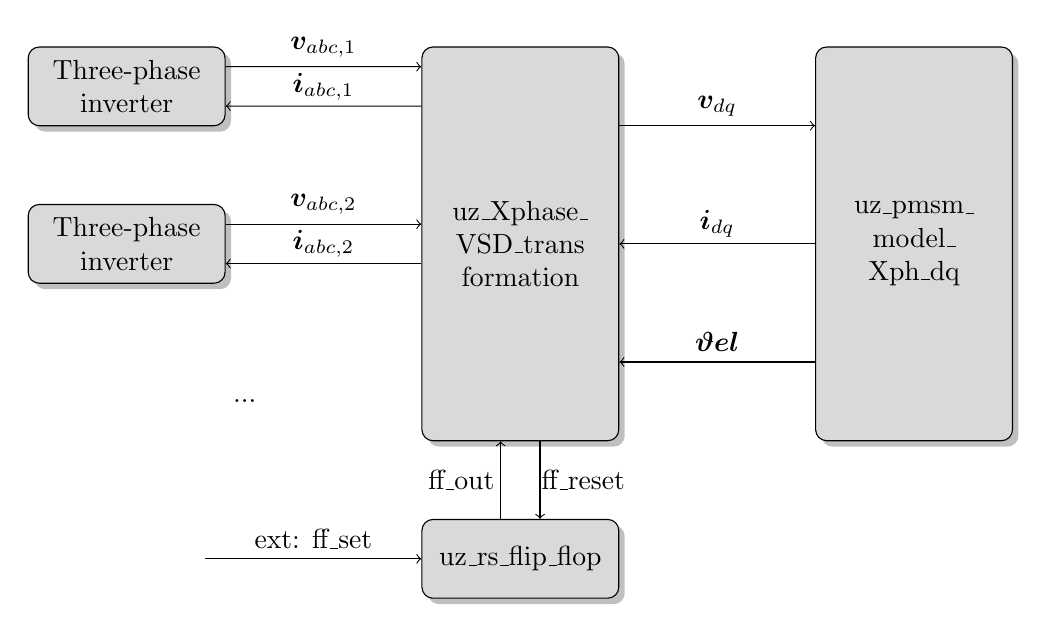
\begin{tikzpicture}% Example:
			\usetikzlibrary{backgrounds}
			\usetikzlibrary{shadows}
			\tikzstyle{big} = [rectangle, rounded corners, minimum width=2.5cm, minimum height=5cm,text centered, draw=black, fill=gray!30, align=center,drop shadow]
			\tikzstyle{small} = [rectangle, rounded corners, minimum width=2.5cm, minimum height=1cm,text centered, draw=black, fill=gray!30, align=center,drop shadow]
			
			
			
			\node (inverter1) [small, yshift=2cm] {Three-phase\\inverter};
			\node (inverter2) [small,] {Three-phase\\inverter};
			
			\node (inverterplaceholder) [yshift=-2cm, xshift=1.5cm] {...};
			
			\node (transformation) [big, xshift=5cm] {uz\_Xphase\_\\VSD\_trans\\formation};
			\node (fliflop) [small, xshift=5cm, yshift=-4cm] {uz\_rs\_flip\_flop};
			
			\node (pmsm) [big, xshift=10cm] {uz\_pmsm\_\\model\_\\Xph\_dq};
		
			\draw[->] ([yshift=0.25cm]inverter1.east) -- node[yshift=0.25cm] {$\bm{v}_{abc,1}$} ([yshift=2.25cm]transformation.west);
			\draw[->] ([yshift=1.75cm]transformation.west) -- node[yshift=0.25cm] {$\bm{i}_{abc,1}$} ([yshift=-0.25cm]inverter1.east);
			\draw[->] ([yshift=0.25cm]inverter2.east) -- node[yshift=0.25cm] {$\bm{v}_{abc,2}$} ([yshift=0.25cm]transformation.west);
			\draw[->] ([yshift=-0.25cm]transformation.west) -- node[yshift=0.25cm] {$\bm{i}_{abc,2}$} ([yshift=-0.25cm]inverter2.east);
			
			\draw[->] ([xshift=-0.25cm]fliflop.north) -- node[xshift=-0.5cm] {ff\_out} ([xshift=-0.25cm]transformation.south);
			\draw[->] ([xshift=0.25cm]transformation.south) -- node[xshift=0.55cm] {ff\_reset} ([xshift=0.25cm]fliflop.north);
			\draw[->] (1cm,-4cm) -- node[yshift=0.25cm] {ext: ff\_set} (fliflop.west);
						
			\draw[->] ([yshift=1.5cm]transformation.east) -- node[text width=1cm, align=center, yshift=0.25cm] {$\bm{v}_{dq}$} ([yshift=1.5cm]pmsm.west);
			\draw[->] ([yshift=0]pmsm.west) -- node[text width=1cm, align=center, yshift=0.25cm] {$\bm{i}_{dq}$} ([yshift=0]transformation.east);
			\draw[->] ([yshift=-1.5cm]pmsm.west) -- node[text width=1cm, align=center,yshift=0.25cm] {$\bm{\vartheta{el}}$} ([yshift=-1.5cm]transformation.east);
			
	\end{tikzpicture}
\end{document}